% Native dvisvgm paths for latex; preserve the PDF driver for pdflatex.
\ifdefined\pdfoutput
  \ifnum\pdfoutput=0 \def\pgfsysdriver{pgfsys-dvisvgm.def}\fi
\fi
\documentclass[tikz,border=8pt]{standalone}
\usepackage{amsmath,amssymb}
\usetikzlibrary{arrows.meta}
\definecolor{positive}{HTML}{C66A20}
\definecolor{negative}{HTML}{2773B4}
% Reusable triple-line Yang--Baxter geometry and edge-state arrows.
% Arguments: horizontal mirror (+1/-1), descending-diagonal arrow style,
% rising-diagonal arrow style, show vertex markers (0/1), right-leg extension.
\providecommand{\abaYBEVerticalArrow}{->}
\newcommand{\abaYBETriple}[5]{%
  \begin{scope}[xscale=#1]
  \pgfmathsetmacro{\abaYBEXEnd}{1.15+#5}
  \pgfmathsetmacro{\abaYBEYEnd}{.95+.6875*#5}
  \draw[\abaYBEVerticalArrow] (.65,-1.4)--(.65,1.4);
  \draw[#2] (-1.25,.7)--(\abaYBEXEnd,-\abaYBEYEnd);
  \draw[#3] (-1.25,-.7)--(\abaYBEXEnd,\abaYBEYEnd);
  \ifnum#4=1
    \fill (.65,-.60625) circle (2.7pt);
    \draw[fill=white] (.65,.60625) circle (2.7pt);
  \fi
  \end{scope}%
}
% Boundary indices in clockwise positions, starting at upper left and then
% lower left, top, bottom, upper right, lower right.
\newcommand{\abaYBEBoundaryLabels}[6]{%
  \node[anchor=east] at (-1.28,.73) {$#1$};
  \node[anchor=east] at (-1.28,-.73) {$#2$};
  \node[anchor=south] at (.65,1.48) {$#3$};
  \node[anchor=north] at (.65,-1.48) {$#4$};
  \node[anchor=west] at (1.19,.98) {$#5$};
  \node[anchor=west] at (1.19,-.98) {$#6$};
}
% An edge-state arrow located on an existing strand, retaining its direction.
% Arguments: center x,y; direction dx,dy; semantic color.
\newcommand{\abaStateArrow}[5]{%
  \pgfmathsetmacro{\abaArrowNorm}{sqrt((#3)^2+(#4)^2)}
  \pgfmathsetmacro{\abaArrowDX}{.09*(#3)/\abaArrowNorm}
  \pgfmathsetmacro{\abaArrowDY}{.09*(#4)/\abaArrowNorm}
  \draw[#5,-{Stealth[length=7pt,width=7pt]}]
    ({#1-\abaArrowDX},{#2-\abaArrowDY})--({#1+\abaArrowDX},{#2+\abaArrowDY});
}

% Spectral labels follow the three intersections; mirror placement with geometry.
% Arguments: mirror (+1/-1), upper-vertex label, lower-vertex label, bare label.
\newcommand{\abaYBEParameterLabels}[4]{%
  \ifnum#1=1
    \node[anchor=east] at (.50,.75) {$#2$};
    \node[anchor=east] at (.50,-.75) {$#3$};
    \node[anchor=east] at (-.42,0) {$#4$};
  \else
    \node[anchor=west] at (-.50,.75) {$#2$};
    \node[anchor=west] at (-.50,-.75) {$#3$};
    \node[anchor=west] at (.42,0) {$#4$};
  \fi
}

\begin{document}
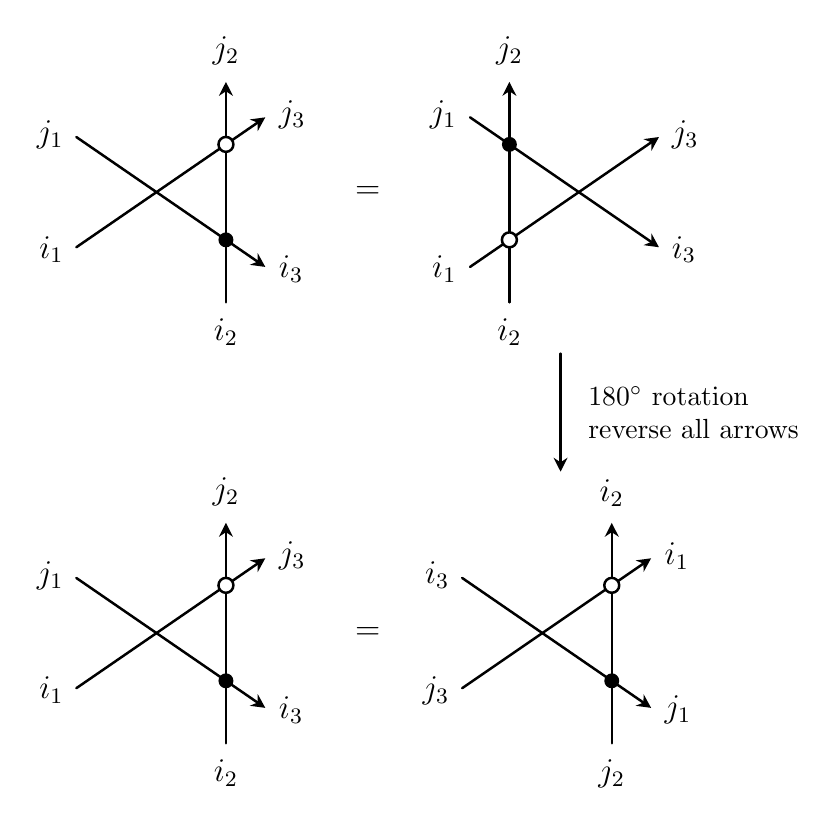
\begin{tikzpicture}[font=\large,line width=.9pt,>={Stealth[length=5pt,width=5pt]},line cap=round,line join=round]
% The upper equation is the earlier YBE, now with boundary indices.
\abaYBETriple{1}{->}{->}{1}{0}
\abaYBEBoundaryLabels{j_1}{i_1}{j_2}{i_2}{j_3}{i_3}
\node at (2.45,0) {$=$};
\begin{scope}[xshift=4.9cm]
  % The two RHS layouts track vertex identities and boundary indices
  % through the half-turn. Arrowheads denote the diagram reference directions.
  \begin{scope}[rotate=180]
    \renewcommand{\abaYBEVerticalArrow}{<-}
    \abaYBETriple{1}{<-}{<-}{1}{0}
  \end{scope}
  \node[anchor=east] at (-1.19,.98) {$j_1$};
  \node[anchor=east] at (-1.19,-.98) {$i_1$};
  \node[anchor=south] at (-.65,1.48) {$j_2$};
  \node[anchor=north] at (-.65,-1.48) {$i_2$};
  \node[anchor=west] at (1.28,.73) {$j_3$};
  \node[anchor=west] at (1.28,-.73) {$i_3$};
\end{scope}
% Only the right-hand diagram is transformed; the left stays fixed.
\draw[->] (4.9,-2.05)--(4.9,-3.55);
\node[anchor=west,align=left,font=\normalsize] at (5.12,-2.8)
  {$180^\circ$ rotation\\reverse all arrows};
\begin{scope}[yshift=-5.6cm]
  \abaYBETriple{1}{->}{->}{1}{0}
  \abaYBEBoundaryLabels{j_1}{i_1}{j_2}{i_2}{j_3}{i_3}
  \node at (2.45,0) {$=$};
  \begin{scope}[xshift=4.9cm]
    \abaYBETriple{1}{->}{->}{1}{0}
    \abaYBEBoundaryLabels{i_3}{j_3}{i_2}{j_2}{i_1}{j_1}
  \end{scope}
\end{scope}
\end{tikzpicture}
\end{document}
